\documentclass[11pt,twocolumn]{article}
\renewcommand{\thesection}{\Roman{section}}
\renewcommand{\thesubsection}{\thesection.\Alph{subsection}}
\usepackage[utf8x]{inputenc}
\usepackage{ifpdf}
\usepackage{multicol}
\usepackage{placeins}
\usepackage{qtree}
\usepackage{fancyhdr}
\usepackage{cite}
%\renewcommand{\cite}{\textcolor{red}}
\usepackage{url}
\usepackage[english]{babel}
\usepackage{amsmath}






\ifpdf 
    \usepackage[pdftex]{graphicx}   % to include graphics
    \pdfcompresslevel=9 
    \usepackage[pdftex,     % sets up hyperref to use pdftex driver
            plainpages=false,   % allows page i and 1 to exist in the same document
            breaklinks=true,    % link texts can be broken at the end of line
            colorlinks=true,
            linkcolor=blue,
            citecolor=blue,
            pdftitle=Lego Car Documentation
           ]{hyperref} 
    \usepackage{thumbpdf}
\else 
    \usepackage{graphicx}       % to include graphics
\usepackage{color}
\usepackage[colorlinks=true,
        linkcolor=blue, citecolor=blue]{hyperref}

\fi 
\usepackage{tikz}

\pagestyle{fancy}
\fancyhf{}
\lhead{\hspace{.5cm} Abdallah Attawia, Moritz Dötterl, Heiko Lengenfelder, Berkay Sümer}
\rhead{Lego Car \hspace{.5cm}}
\cfoot{\thepage}
\onecolumn
\title{\textbf{Lab Course: Hardware/Software Co-Design with a LEGO Car\\[3ex]}
\normalsize{\center{\textbf{\LARGE{SS 16}}}\\ 
\textbf{Abdallah Attawia, Moritz Dötterl, Heiko Lengenfelder, Berkay Sümer} \\
%Matriculation Number: 03664889} \\[3ex]
Technische Universität München, Garching, Department of Informatics \\
Boltzmannstr. 3, 85748 Garching, Germany  \\
%e-mail address: abdallah.attawia@tum.de \\[3ex] 
\begin{flushleft}
This document explains the work done on a lego car to detect and follow a line autonomously. Connection and communication between the hardware parts is explained. Furthermore, collision avoidance and line detection algorithms are thoroughly described.    
\end{flushleft}
}}

\twocolumn

\begin{document}
\date{}
\maketitle
\tableofcontents
\newpage
\noindent
\section{Introduction}
An autonomous car is one that can drive from point A to B independently without any human input. It can accelerate, brake and steer itself as well as sense the environment and navigate to avoid crashing. The development of autonomous vehicles is rapidly growing and a lot of big and small companies are working towards making autonomous driving a reality.\\
In this project a small scaled model, a lego car, along with some cheap components are used to test a real autonomous driving function, i.e. following a line on the street. This documentation starts with a brief explanation of the different hardware components. Then the cabling and communication between the components is described. Lastly, the collision avoidance technique and and the line detection and following are explained. The code, attached to this report, carries out the functions explained here and is clearly documented.
\section{Components overview} 
The hardware components used are two controllers, the DEO-Nano and the Raspberry Pi, two types of actuators, namely speed motors and servo motors, as well as two types of sensors, which are the ultrasound sensors and the USB-camera.
\subsection{DEO-Nano} 
The DE0-Nano board is a compact-sized FPGA based development platform manufactured by terasIC. Its heart is a Cyclone IV FPGA from Altera. Furthermore it features on board memory, LEDs, Buttons, and most importantly three GPIO headers. On this FPGA we flashed the provided Nios-II image. This is an image of an adaptable processor allowing for custom specializations such as multiple hardware UART handlers. Now it is possible to wright code for this processor in C using the hardware you desire, without any trade off. We are using four UART units to connect to three ultrasonic sensors as well as to the Raspberry Pi. Furthermore we use two PWM modules with each two channels allowing us to generate PWM signals at four pins. Those are used to control the drive motor and the steering servo.
\subsection{Raspberry Pi}
For this project the newly released Raspberry Pi 3 is used. Raspberry Pi is a small-sized one board computer. In this work it is used to connect the camera with the Nano-board and to run the line following code.\\
First, the micro SD-card for the Pi is prepared with the Raspbian Operating System installed on it. Then the Pi is boots the Raspbian and the computer is connected to the Raspberry Pi using Secure Schell (SSH) either via the Ethernet port, or using the build in Wi-Fi of the Pi 3 and the LRZ Wi-Fi network. Then the camera is connected using one of the USB ports and OpenCV is installed to run the line following code. Finally UART communication is enabled to connect the Raspberry Pi with the Nano-board. In Raspberry Pi 3 you need to disable Bluetooth in order for UART communication to work. To disable onboard Pi3 Bluetooth and restore UART over GPIOs 14 and 15, modify the file "/boot/config.txt":
\begin{itemize}
\item {sudo nano /boot/config.txt}
\item {Add to the end of the file: \\"dtoverlay=pi3-disable-bt"}
\end{itemize}
\subsection{Actuators}
\subsubsection{Speed motors}
The car has two Lego based driving motors that control the speed of the car. The motors are wired together to act as one motor, but with double the power. One motor drives the front tires, the other motor the rear tires to provide maximum traction.
\subsubsection{Servo motor}
The car uses one Lego servo motor to steer the direction. The servo steers both axles of the car to provide maximum agility and a relatively low turning cycle.
\subsection{Sensors} 
\subsubsection{Ultrasound sensor}
The ultrasound sensor measures the distance from any detected object within its range. As shown in Figure \ref{ultrasound} the ultrasound sensors detects objects by sending out ultrasound waves and receiving an echo, if an object is detected. The sensor measures the time of flight between transmitting and receiving the signal and calculates the distance according to the following formula (\ref{dis}).
	
\begin{equation}
\centering
L = \frac{340(m/s)x\bigtriangleup t(s)}{2}
\label{dis}
\end{equation}

\begin{figure}[h]
\centering
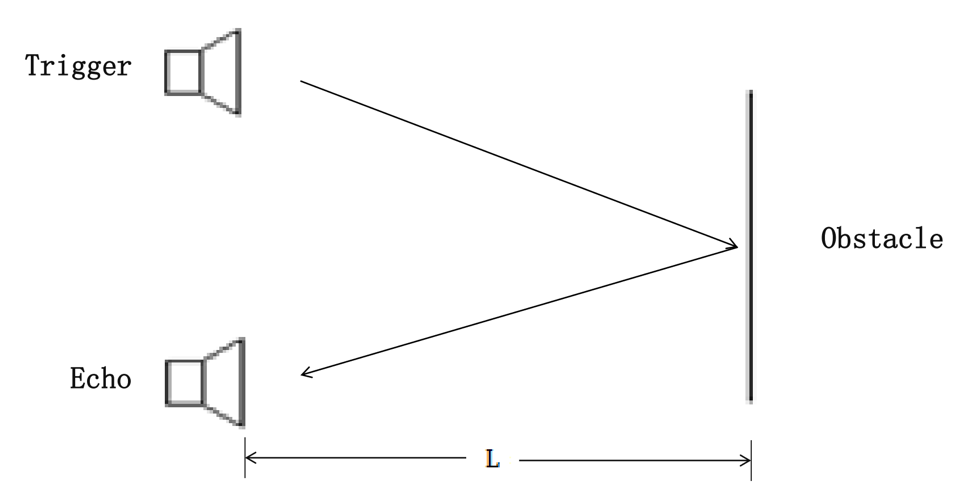
\includegraphics[width=0.5\textwidth]{ultrasound.png}
\caption{Theory of operation of the ultrasound sensor}
\label{ultrasound}
\end{figure}

In this course, the KS103 ultrasound sensor is used. It has a range up to 11m which can be specified by sending a command from the Nano-board. This sensor can operate using two digital communication protocols; I2C and Uart. It has an accuracy between $1mm$ and $10mm$\\
In order for the ultrasound sensor to operate, it is first initialized and set to the desired range. Like the raspberry pi, it communicates with the Nano-board using uart communication, which has to be initialized as well. The Nano-board then sends a command to the sensor to send the data using uat. The Nano-board finally receives date from the sensor. The data read from the sensor is multiplied times 170 to get the distance from detected objects in micrometer.  
\subsubsection{USB Camera}
A standard USB web cam is used to provide a stream of images of the area in front of the car. How these images are processed is explained in chapter \ref{ImProLinFol}.

\section{Hardware}
we used several different devices to build up our Lego Car. This chapter explains what devices we have used, and how they are interconnected.
\subsection{Components}
The Hardware can be divided into four sub groups listed below:\\
\newpage
\textbf{Power Supply}
\begin{itemize}
	\item Battery
	\item H-Bridge
	\item CPT 15W DC/DC Converter
\end{itemize}
\textbf{Sensors}
\begin{itemize}
	\item KS103 Ultrasound Sensor
	\item Camera
\end{itemize}
\textbf{Control}
\begin{itemize}
	\item DE0-Nano Board
	\item Raspberry Pi 3 
\end{itemize}
\textbf{Actuators}
\begin{itemize}
	\item Steering Servo Motor
	\item Drive Motors
\end{itemize}
\begin{figure*}[h]
\centering
\includegraphics[width=\textwidth]{wiringDiagram.png}
\caption{wiring diagram of the car}
\label{wiringDiagram}
\end{figure*}
Figure \ref{wiringDiagram} shows the wiring diagram of the total car setup. Including the Ultrasound sensor, the Nano Board, the steering servo, the driving motor in the first row (from left to right) and the USB Camera, the Raspberry Pi, the DC/DC converter and the battery in the second row (also from left to right). The H-Bridge is shown between those two rows and the wiring is depicted as colored lines interconnecting all devices.


\subsection{Power Supply}

As a power source, we are using a three cell LIPO battery called “eco-x 5000 Top Fuel” which provides 11.1V. An H-Bridge with integrated voltage divider is used to convert from battery voltage to 5V to power the Nano Board which works at 5V. Furthermore the H-Bridge is used to translate the 5V signals from the Nano Board to 11.1V signals for the Drive Motor. We are also using a DC/DC converter which is an electronic circuit that also converts from the battery voltage to 5V. It is used to power the Raspberry Pi, since the voltage divider of the H-Bridge is not powerful enough for the Raspberry Pi. To ensure all devices work together they are all connected to the common Ground of the battery.


\subsubsection{Power Connection}

The 11.1V red cable of the battery is connected with the VCC input of the H-Bridge, and with the red cable of the DC/DC converter. The black GND cable of the battery is connected with the GND input of the H-Bridge, and the black ground input of the DC/DC converter.\\
The 5V input of the Nano Board is connected to the 5V Output of the H-Bridge, alternatively it could also be wired to the 5V output of the DC/DC converter. The GND of the Nano board is connected to the Ground of the whole car, e.g at the GND input of the H-Bridge\\
The servo motor's 11.1V input is attached to the VCC input of the H-Bridge. GND input of the servo motor has to be connected with the common Ground, so the GND input of the H-Bridge.


\subsection{Sensors}

A simple web cam and one “KS103" ultrasound sensor are used as sensors. In principle we got three ultrasound sensors, but we only needed one to get the distance to objects in front of the car. so this document will only focus on the single sensor.Based on this sensor the car will adopt it's speed. How this is done exactly is discussed in \ref{Usensor}. The camera is used for the line detection which is discussed in chapter \ref{ImProLinFol}.\newpage
The KS103 Ultrasound Module has 5 pins (listed from right to left):
\begin{itemize}
\item VCC: power pin
\item SDA/TX: data pin ($I^2C$) / Transmitter pin UART
\item SCL/RX: clock pin ($I^2C$) / Receiver pin UART
\item GND: power ground pin
\item Mode: selects the communication mode (UART or $I^2C$)
\end{itemize}
There are two options for the communication: UART (universal asynchronous receiver/transmitter) and $I^2C$. Depending on the status of the Mode pin the sensor either expects $I^2C$ (Mode pin high), or UART (Mode pin low) communication. We are using the UART modus in this project, which is an asynchronous serial communication format.

\subsubsection{Sensor Connection}
The 5V VCC and GND pins of the sensor are connected with the 5V and GND pins on the GPIO header of the Nano Board to power the sensor.\\
The Mode pin has to be connected with a GND pin of the Nano Board to select the UART mode.\\
The TX and RX pins of the sensor are connected to the UART pins of the Nano Board. Note that, as usual with UART, the TX pin of the sensor is connected to the RX pin of the Nano Board and vice versa. GPIO\_00 is connected with the TX pin of the sensor and GPIO\_01 with the RX pin of the sensor.\\
The camera is simply plugged into one of the USB-ports of the Raspberry Pi.

\subsection{Control}

We are using the “DE0-Nano Board” to provide an interface for the “Raspberry Pi 3” to control the car. The DE0-Nano Board introduces a compact-sized FPGA development platform suited for portable design projects, such as robots and mobile projects. A UART connection is used to enable communication between these two Boards. The calculation for the steering is done on the Raspberry Pi while the Nano Board generates the signals for the actuators and handles the connection to the ultrasonic sensor.

\subsubsection{Control Connection}
The UART pins of the Pi are connected with the UART pins of the Nano Board. The 8th pin of the Pi is the TX and 10th pin is the RX pin. They are connected to GPIO\_016 and GPIO\_017 of the Nano Board respectively.\\
The 2nd and 4th pins of the Pi are two 5V pins which can be used to power the Pi itself, or power other small devices from the Pi. Either one of them is connected with the the 5V output of the DC/DC converter. The 6th pin is the GND pin which has to be connected with the GND of the care e.g. the GND output of the DC/DC converter.

\subsection{Motors}

We have two driving motors connected in a parallel manner and one servo motor on our car. The servo is used for the steering and the two driving motors are used to move the car. We are using PWM(Puls-width modulation) to generate analog control signals for the Motors. By using this modulation we had the ability to arrange the speed of our car and also the steering angle. The speed is adjusted by setting one pin of the driving motor to ground and generating a PWM signal on the other pin. The duty cycle of the PWM determines the speed of the car while switching the PWM and the ground pin causes the car to drive in the other direction. So setting one pin to '0' and the other pin to '1' would result in maximum speed while setting the pins to '1' and '0' would result in maximum reverse speed. The steering servo basically works the same way except that not the number of revolutions per time is controlled, but the angle of the servo. So setting the control pins to '0' and '1' respectively will cause the servo to steer all the way to one side, while setting the pins to '1' and '0' will make the servo steer all the way to the other side. 

\subsubsection{Motors Connection}
The driving motors are both connected together, so they work as if we had one motor. The two pins of the motor are connected to the high voltage output of the H-Bridge. We are using OUT3 and OUT4 of the H-Bridge. The PWM output of the Nano Board is connected to the according low voltage input of the H-Bridge. We are using GPIO\_112 and GPIO\_113 on the Nano Board and connected them with IN3 and IN4 of the H-Bridge. Now the H-Bridge will transfer our signals to the 11.1V logic level the driving motor needs. Furthermore the high currencies needed by the motor will not flow through the Nano Board, which would be destroyed by them.\\
The two remaining cables of the servo motor are directly connected to the PWM output pins GPIO\_114 and GPIO\_115 of the Nano Board. Here no conversion between different logic levels is necessary and no high currencies could harm the Nano Board.


%\section{Communication}

\section{Collision Avoidance}
\label{Usensor}
In order to avoid collisions, an algorithm based on the idea of the adaptive cruise control is implemented. Adaptive cruise control is a cruise control function that allows the vehicle to adapt its speed according to the traffic and to maintain a safe distance from the vehicles ahead.\\
In real cars, a long range radar sensor is used to detect the cars, here we use an ultrasound sensor to measure the distance from the vehicles ahead. The following algorithm is implemented to avoid the collision with other cars or objects and to adapt the speed to the surrounding traffic.
\begin{itemize}
	\item if distance from ultrasound sensor $\leq$ a minimum set distance ($distance_{min}$)\\
	-car stops
	\item if distance from ultrasound sensor $\geq$ a maximum set distance ($distance_{max}$)\\
	 -drive with maximum speed
	\item else (distance lies within $distance_{min}$ and $distance_{max}$)\\
	 -adapt speed according to distance:\\
	 \begin{equation}
	 CurSpeed = MaxSpeed * \frac{distance}{distance_{max}}
	 \end{equation}
\end{itemize}
The speed of the car is set according to the aforementioned algorithm, where the current speed is the duty cycle that is assigned to the speed motors.
\section{Image processing for line detection and following}
\label{ImProLinFol}
The task of the whole project was to build a Lego Car that can autonomous follow a line on the ground. For this purpose we are using an ordinary web cam on the front of the car giving us an image of the ground up to approximately 20 cm in front of the car. We developed an algorithm that detects the line in the image and calculates how the car needs to steer in order to stay on that line. The calculation is entirely done on the Raspberry Pi using the image processing framework OpenCV. The following sections explain how the image processing works and how we optimized it for the Raspberry Pi.

\subsection{Code}
%\subsection{Code}
%\subsection{Optimization}
\subsubsection{Sequential Improvements}
Having this basic concept of the algorithm implemented we needed to test it of course. But our first tests where not so successful, the car lost the line quite often. To prove our concept we replaced the Pi with an ordinary laptop, using a USB UART adapter. With this setup the algorithm turned out to be working really good, and the car stayed on the line every time, even with the driving motor running at full speed. The main difference between those two setups is the computation power, which is obviously way higher on the laptop than on the Raspberry Pi. After some performance analysis we figured out that the computation of a single frame takes around 4 ms on the laptop and 170 ms on the Raspberry Pi.
We also figured out that our camera gives us 15 frames per second (FPS), so a new image is provided approximately every 66 ms. This means that we are only processing every third image on the Raspberry Pi and that is the reason for the poor performance. So there are two things to be done: first of all shorten the calculation time per image and second make sure every frame of the camera is processed and therefor really used, so we are no longer wasting information. Improving the calculation time also improves our reaction time, since thats exactly the time it takes to get an image of an event (e.g. an approaching turn) and to calculate what the car should do. So the faster the computation time is the faster the car can drive. Ensuring every frame gets calculated does not improve the reaction time, but it improves the overall throughput and therefor every 66 ms a new steering angle would be present. This also improves the feasible speed of the car.\\
To save computation time we disabled the software Gaussian Filter. It turned out that it can be easily replaced by changing the focus of the camera, so it produces a blurred image. That is exactly the same thing the Gaussian Filter would do, but in hardware rather than in software. It can be seen, that a sharp image without Gaussian Filter makes the algorithm very vulnerable to noise, but as soon as the focus of the camera is changed the algorithm recognizes the line without problems. \\
Another optimization is that the search range is restricted. Before the whole row of the image was searched for the highest gradient, now only the area of the X-Position found in the row below $\pm80$ Pixels is searched. The highest gradient is assumed to be on the line. This assumption is reasonable, since the line always is continuous and won't change so fast. This method only works if the pixel found in the lowest row of the image is on the line, and not noise. In reality this turned out to not be a problem since if there is a correct line on the image it needs also to be in the lowest row of the image and it is identified correctly.\\
Furthermore only gradients grater than 25 are considered. This helps to recognize if the line has left the image to either the left or the right side of the image. In those cases it is possible that a row has no pixel on the line and therefor no gradient grater than 25. In this case the coresponding line gets neglected, saving further computation time due to less points on the line. Even more important is that this makes the algorithm less vulnerable to noise in the case that the line leaves the image to one of the sides. Without this any random noise above the point where the line leaves the image would be interpreted as the line and affect the steering calculations in a bad way.\\
With all these improvements we managed to bring the computation time down to approximately 100 to 110 ms per frame, which is pretty good, but still not good enough to capture all frames. But that approach only uses one core of the four cores the Raspberry Pi provides.
\subsubsection{Exploit Parallelism}
Since it is not possible to catch every frame of the camera with just one thread on the Raspberry Pi we need to exploit the parallelism of the Pi. So we first tried to make OpenCV use OpenMP to parallelize it's computations. That seemed to work, it brought the computation time per frame down to 80 ms. But that is still not faster than the 66 ms latency of the camera. So still further improvements need to be done. But since this implicit parallelism seems not to work well together with the explicit parallelism described in the next part we had to deactivate the OpenMP version again.\\
So we developed our own way to make use of the four cores the Raspberry Pi has. The idea is to use multiple threads that each grab a frame, process it and propagate the resulting steering angle to the UART output and the Nano board. With one computation taking 100 to 110 ms two threads are sufficient to calculate each image. The way this works is as follows: \\
The main thread creates two worker threads and sleeps then. The worker threads grab the next frame generated by the camera in a synchronous way, meaning one image is always processed by only one thread. Now the thread processes the image and calculates the steering angle. After that the thread performs a check whether the calculated frame is still in the same order than the sequential stream of images. If not, e.g. the calculation of this frame took to long and the next frame has already finished, it is neglected. Usually this is not the case, since the frames all approximately take the same amount of time to be computed. Than the worker thread wakes the main thread through a condition variable and propagates the calculated steering angle. While the worker waits for the next frame of the camera the main thread generates the UART output and sends the calculated steering angle to the Nano board. The main thread starts to sleep again, while the worker thread continues to process the next image.\\
With this technique the worker threads alternately grab the images provided from the camera, all frames are used and no information is wasted. Since the Raspberry Pi has four cores this method could also be run with four worker threads instead of just two. In our case, there is nothing to gain by using four threads rather than two, since the camera only produces 15 FPS. So for example with three threads one thread would always be waiting, so the algorithm degenerates to the two thread version. But if a different camera with 30 FPS would be used it would be helpful to use four worker threads. This way even all the 30 FPS could all be calculated and used for the line detection. Figure \ref{SequenzDiagram} shows how all images of the camera can be calculated using two threads. Note that the time between two images and the time for calculating one image is on scale. For simplicity this shows only a part of the whole program and only the necessary communication. It can be seen that after each computation there is enough time for the thread to wait for the next image.

\begin{figure}
\centering
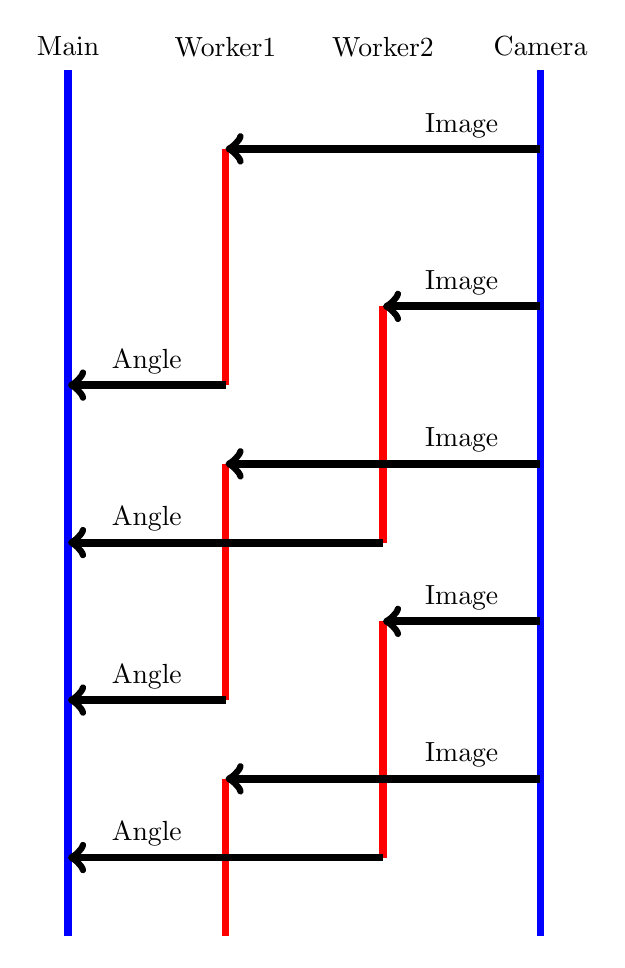
\begin{tikzpicture}
    \draw[line width=1mm, color = blue] (-3,0) -- (-3,-11) (3,0) -- (3,-11);
    \draw[line width=1mm, color = red] (-1,-1) -- (-1,-4) (1,-3) -- (1,-6);
    \node at (-3,.3) {Main};
   % \node at (-3,-3) {Sleeping};
    \node at (-1,.3) {Worker1};
    \node at (1,.3) {Worker2};
    \node at (3,.3) {Camera};
  %  \draw[->] (-3,-1) -- node[midway,above] {create()} (-1,-1);
  %  \draw[->] (-3,-2) -- node[midway,above] {create()} (1,-2);
   % \draw[->] (-1,-3) -- node[midway,above] {GetImage()} (3,-3);
   % \draw[->] (1,-4) -- node[midway,above] {GetImage()} (3,-4);
    \draw[<-,line width=1mm] (-1,-1) -- (3,-1);
    \node at (2,-0.7) {Image};
   % \node at (-1,-6) {Processing};
    \draw[line width=1mm, color = red] (-1,-5) -- (-1,-8) (-1,-9) -- (-1,-11) (1,-7) -- (1,-10);
    \draw[<-,line width=1mm] (1,-3) --(3,-3);
    \node at (2,-2.7) {Image};
    \draw[<-,line width=1mm] (-3,-4) -- (-1,-4);
    \node at (-2,-3.7) {Angle};
    \draw[<-,line width=1mm] (-3,-6) -- (1,-6);
    \node at (-2,-5.7) {Angle};
    %\draw[->] (-1,-8.2) -- node[midway,above] {GetImage()} (3,-8.2);
    \draw[<-,line width=1mm] (-1,-5) -- (3,-5);
    \node at (2,-4.7) {Image};
    \draw[<-,line width=1mm] (1,-7) -- (3,-7);
    \node at (2,-6.7) {Image};
    \draw[<-,line width=1mm] (-3,-8) -- (-1,-8);
    \node at (-2,-7.7) {Angle};
    \draw[<-,line width=1mm] (-1,-9) -- (3,-9);
    \node at (2,-8.7) {Image};
    \draw[<-,line width=1mm] (-3,-10) -- (1,-10);
    \node at (-2,-9.7) {Angle};
    
\end{tikzpicture}
	
  \caption{Multithreaded calculation}
  \label{SequenzDiagram}
\end{figure}


\section{Conclusion}
To conclude, the car followed a closed track without getting out of line in both directions. The maximum set speed was about 85\% of the maximum possible speed. With a few modifications on the camera, e.g. a higher frame rate of 30 FPS, or a wider viewing angle, or a higher computation power on the Raspberry Pi, the full motor speed could had been reached.

%\section*{Acknowledgments}


%\begin{small}
%\bibliography{mybib}
%\bibliographystyle{ieeetr}
%\end{small}

\end{document}
